
\documentclass{article}

\usepackage{hyperref}
\usepackage{tabularx}
\usepackage{gantt}

\hypersetup{
    colorlinks=true, %set true if you want colored links
    linktoc=all,     %set to all if you want both sections and subsections linked
    linkcolor=black,  %choose some color if you want links to stand out
}

\title{EPQ Writeup}
\date{}
\author{James Rand}

\def\tightlist{}

\makeatletter
\def\@seccntformat#1{%
    \expandafter\ifx\csname c@#1\endcsname\c@section\else
    \csname the#1\endcsname\quad
      \fi}
\makeatother

\begin{document}


\maketitle

\tableofcontents
\setcounter{tocdepth}{5}

\newpage

\section{Introduction}
\subsection{Objective}

In this extended project I plan to design a device that will be able to interact with a file
server. This device must be able to acheive some of the following functions:

\begin{itemize}
    \item Be able to turn the server on and off
    \item Be power efficient so the running cost is low
    \item forward a shell connection onto the server
    \item Do not exceed the budget of \$50
\end{itemize}

The first object that I wish to discuss is having the ability to remotely turn on and off the
server. This could be done in two ways: the first would be to use wake on lan which would be 
a way of doing it through software; the second is using electrical components to act as an
electric switch. \\

The first approach I would like to talk about is using wake on lan. This seems to be the default
way of doing what I am proposing which means that setting this up will be straight forward and
well documented. The only problem with using this method is that the server will constantly need
to be on standby which conflicts with my second goal of this project being power efficient. The
second approach is the opposite of the first as it will be more difficult to set up due to the 
fact it will require me to buy parts which need to be appopiate to interact the server. On the
plus side though it could be a more power efficient as I could design it to control the mains
power supply as well so that it will not need to be on standby.

\subsection{Time scale}

Since I have a limited amount of time to acheive my goal I have created the following Gante
chart (Fig ~\ref{fig:Gantt Chart}) to illustrate how I intend to use my time. This chart
only shows how I will use the time up to the initial draft. There is time availiable after
this draft but I would like to use this time to improve my write up and act upon feedback.

\begin{figure}  
    \begin{gantt}[xunitlength=\textwidth / 16]{7}{16}
        \begin{ganttitle}
            \titleelement{Number of weeks}{16}
        \end{ganttitle}
        \begin{ganttitle}
            \numtitle{1}{1}{16}{1}
        \end{ganttitle}
        \ganttbar{Research}{0}{7}
        \ganttbarcon{Design}{7}{2}
        \ganttbarcon{Building}{9}{4}
        \ganttbarcon{Reflection}{13}{3}
        \ganttmilestone[color=cyan]{Draft deadline}{16}
        %\ganttmilestonecon{A connected Milestone}{7}
    \end{gantt}
    \caption{Gantt chart} \label{fig:Gantt Chart}
\end{figure}  

\break
\section{Reseach}
\subsection{choosing the right board}

The very first thing that I need to consider when designing this is what development board
I will as everything else will be dependant upon this. The 4 factors that I decided would
be most important to consider are: the price of the board; how easy it would to connect
and control through the internet and power consumption. 

The reason I think power consumption should be something to consider is that this board will
be on for long periods of time to make sure that the server is always available. Which means
running a power hungry device will be expensive and not pratical. The price is an obvious
important feature and since I may be buying extra hardware components I need to be extra wary of
the cost of the board. Since I will be controlling the board through the internet it needs to
have internet connectivity and be straightforward to setup. Finally I need to think about the
implications of the hardware. This means the board must be able to communicate to hardware from
a custom written program.

\subsubsection{Raspberry Pi}

The Raspberry Pi is definatly one of the more well known development boards that are use
extensively by hobbyists. This means that the Raspberry Pi will be well documented so if
I come across any difficulties it will be easier to troubleshoot. The table below compares
the technical specs of all of the models. \\

\begin{tabularx}{\textwidth}{| X | X | X | X | X |}
    \hline
    Raspberry Pi Model & Model A+ & Model B & Model B+ & Model B 2 \\ \hline
    Price              &  \$19.99  &  \$39.99 &  \$29.99  &  \$39.99   \\ \hline
    Processor Speed    &  \multicolumn{4}{c |}{700 Mhz}  \\ \hline
    Power Consumption  &  \multicolumn{3}{c |}{600mA @ 5V} & 650mA @ 5V \\ \hline
    Memory             &  256MB   & \multicolumn{2}{c |}{512MB} & 1GB \\ \hline
    Storage            &  Micro SD Card &  SD Card & \multicolumn{2}{c |}{Micro SD Card} \\ \hline
    Pins               &  40      &    26  & \multicolumn{2}{c |}{40} \\ \hline
    Coding Languages   &  \multicolumn{4}{c |}{Python} \\ \hline
\end{tabularx}
\newline

Information is gather at this website: https://www.makershed.com/pages/raspberry-pi-comparison-chart
\newline

The characteristics that I have mentioned above make the raspberry effortless to develop on;
mainly because it runs the linux operating system. This means that I can use and run any language
that runs linux givving me a wide range of tools to use. I could also install and use programs that
other people have written. As mention above the raspberry pi is very popular meaning the is a wide
range of hardware extenstion that may make it easier to control external components. 

\subsubsection{BeagleBone Black / BeagleBone Black Wireless}

This section will cover a comparison of features on the BeagleBone Black and the BeagleBone Black Wireless.
The only difference between these boards is that one has bluetooth and wifi while the other has ethernet.
These boards, similar to the raspberry pi, are very popular meaning there is a wide range of documentaion
and addons that can be used although it should be noted that they are not as popular as the raspberry pi.
The table below will give a summery of the features availiable. \\

%\newline
\begin{tabularx}{\textwidth}{| X | X | X |}
    \hline
    BeagleBone Model &  BeagleBone Black  & BeagleBone Black Wireless \\ \hline
    Price            &       \$75         &        \$80               \\ \hline
    Processor Speed  &  \multicolumn{2}{c |}{1GHz}                    \\ \hline
    Power Consumption&  \multicolumn{2}{c |}{210-460mA @ 5V}          \\ \hline
    Memory           &  \multicolumn{2}{c |}{512MB}                   \\ \hline
    Storage          &  \multicolumn{2}{c |}{2GB eMMC}                \\ \hline
    Pins             &  \multicolumn{2}{c |}{2x46 pin headers}        \\ \hline
    Coding Languages &  \multicolumn{2}{c |}{C/C}                   \\ \hline
\end{tabularx}
\newline

Information Gather at https://www.digikey.com/en/product-highlight/t/texas-instruments/beagleboard
\url{https://www.amazon.com/BeagleBone-Black-Wireless-Starter-Kit/dp/B01NGTOX40/ref=sr_1_2?ie=UTF8&qid=1510164000&sr=8-2&keywords=beaglebone+wifi&dpID=51g7KiFRteL&preST=_SY300_QL70_&dpSrc=srch}
\url{https://beagleboard.org/black-wireless}
\url{https://beagleboard.org/black/}
\newline

The first thing that I noticed when researching this board is that it can be pricey but looking
at the specs you can see why. These boards are very similar to the raspberry pi but I thought it
was worth discussing this board as it excels in hardware thanks to it's many pins. Simarly to the
raspberry pi it also runs Linux. The BeagleBone also has lower power consumption than the raspberry
pi. Finally it is worth noting that it uses C/C++ for the programming language which is more difficult
to write in than a language such as Python.

\subsubsection{Audino Uno}

The Audino is a classic development board that instead of the previous two items does not have the linux
operating system. That being said due to it's large poplarity there are a huge number of libraries and 
APIs that you can use. \\ 

\begin{tabularx}{\textwidth}{| X | X |}
    \hline
    Audiono Model    &   Audiono Uno \\ \hline
    Price            &       \$25    \\ \hline
    Processor Speed  &      16MHz    \\ \hline
    Power Consumption&    50mA @ 5v  \\ \hline
    Memory           &      32KB     \\ \hline
    Pins             &       20      \\ \hline
    Coding Languages &     C/C++     \\ \hline
\end{tabularx}
\newline

Information Gather at \url{https://makezine.com/product-review/arduino-uno/}


The specs on the ardunio are considerably lower than the previous two items due to the fact that
the arduino is a microcontroller instead of a size down computer. This means that it consumes less
power and has less features that the other two can offer. There is also a problem with wireless
capabilities on the audino as it has none built in and would require me to buy a WiFi sheild.

\subsubsection{Particle Photon}

This board is much more obscure than the rest of the boards that I have compared. Despite this there
are a lot of attractive charactersitics that this board like the fact that it has in built wireless
and can be communicated with through the internet without the need to port forward. Additionaly this
board is the smallest of all of the ones that I have considered. \\

\begin{tabularx}{\textwidth}{| X | X |}
    \hline
    Particle Model   &    Photon     \\ \hline
    Price            &     \$19      \\ \hline
    Processor Speed  &    120Mhz     \\ \hline
    Power Consumption& 80mA @ 5V-3.3V\\ \hline
    Memory           &    128KB      \\ \hline
    Storage          &     1MB       \\ \hline
    Pins             &     28        \\ \hline
    Coding Languages &    C/C++      \\ \hline
\end{tabularx}
\newline

Informatino Gather at \url{https://makezine.com/product-review/particle-photon/}
\url{https://docs.particle.io/datasheets/photon-(wifi)/photon-datasheet/#power} \\

%\newline

Similarly to the Arduino this board is a microcontroller. The features I mentioned above reagarding
connectivity will make development considerable easier. This is also the cheapest board that I have
compared giving me plenty of left over money to buy all the hardware components that I might need.


\subsubsection{The Board I Chose}

After considering the pros and cons of all of these boards I decided that a microcontroller type 
would be much more suitable for my project. My reasoning behind this is that a fast processor and
a linux operating system is unecessary in this situation meaning that I would be wasting power on
features that I am not going to use. The price is also higher for the non-microcontrollers.

I now needed to make a decision between the Audino and the Particle Photon. Although the arduino has
a huge number of libraires and a comprehensive documentation; I came to the conclus

\subsection{Transitors vs Relays}

In order to interact with the server on a hardware level I need a component that can act like an
electrical switch. This is so that when I need to turn the server on and off I can acheive this with
this "electical switch". There are two components that took my interest while researching this. The
first is transitros which are part of the semiconductor family and are largely used in computers. The
second is a relay which unlike a transitor has moving parts and works using an electro magnet. The first
that I will discuss in detail are transitors.

\subsubsection{Transitors}

\begin{figure}

    The source for this information: \url{https://learn.sparkfun.com/tutorials/transistors}
    
    There are many different types of transistors but the most common and the one I am most interested in is
    the "Bipolar junction transistor" or "BJT" for short. There are two types of BJT that I need to discuss
    which are NPN and PNP. Before I start describing those it is importatnt to understand the basic anotomey
    of transistors first.

    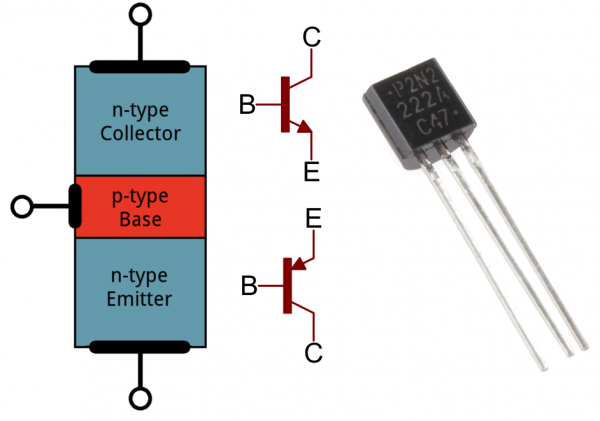
\includegraphics{pictures/transistor-layout.png}
    \caption{transistor layout} \label{fig:transistor-layout}
    \vspace{0.5cm}

    In the layout above (Fig ~\ref{fig:transistor-layout}) you can clearly see that a transitor has three legs.
    These legs each do different things and have special names: collecter, base and emitter. The leg in the middle
    called the base is the one we are most interested in as this can control the current throught the emitter and 
    collector by varying the input to it. The collector and emitter can change based upon the type of transitor

\end{figure}

\begin{figure}
    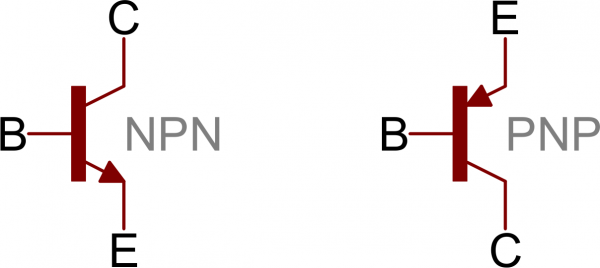
\includegraphics{pictures/npn-pnp-symbols.png}
    \caption{NPN vs PNP} \label{fig:different-transitor-layout}
    \vspace{0.5cm}

    The two different diagrams above show the different types of BJT transitors
    (Fig ~\ref{fig:different-transitor-layout}). \\

    The only difference between these two types which is illustrated by this figure is the direction of the 
    emiiter arrow. This small difference has big implications and lead to different properties for each. I
    will now start to disscuss these consequences and which out of the two I think is most suitable for this
    project.

\end{figure}

\break 

Unlike many other electrical components like resistors and capacitors which have a linear relationship with 
voltage and current transitors have four different ways of handling electrical power:

\begin{itemize}
    \item Saturation     --- Which freely alows volatage and current to flow from the collector to emitter
    \item Cut-off        --- Allows no volatege or current from collector to emitter. Oposite of "Saturation"
    \item Active         --- The current from the collector to emitter is proportional to the current flowing
        through the base
    \item Reverse-Active --- Similar to "Active" the current is proportional to the base but flows in reverse
\end{itemize}

For the purposes of this project the only modes worth discussing are "Saturation" and "Cut-off" because we
are only interested in on or off and not anything inbetween. 

To determine what mode the transistor is in you need to investigate what voltage is supplied to each pin.
In order to put a NPN transistor into staturation mode the volatege supplied to the base, V\textsubscript{B}
needs to be greater that the voltage supplied to the emitter, V\textsubscript{E}. To put into cut-off mode
it needs to be the opposite. Likewise with PNP transistors it is reversed.

After considering these factors I decided to perform an experiment to get use to using transistors. I did
this by connect up an led and transistor to my board and checking that I can turn it off and on by emmitting
an output voltage on one of the pins. A schematic of my experiment can be seen below in figure >>>>>>.



I flash a example program onto the board called "Blinky". The purpose of this program to to turn a output
pin on and off every second. This output pin is labeled the voltage alternator in th diagram. After I
design this circuit I then built it on a bread board which is shown below in figure >>>>>>>. The result
of this is the led turn off and the on again.

\subsubsection{Relay}

An alternative to the transistors is the relay. Similarly to the transistor this can work as an electronic
switch. The main difference between a relay and a transistor is that a relay have physical moving parts
inside. Inside a relay there is an electro magnet which can pull a thin piece of metal down to make the 
switch close. This is how a relay works. Due to this mechanisism a relay can be significantly bigger than
and a transistor it can calso handle higher volatages with ease. A downside to a relay is that it can
take longer for it to switch on and off. Luckly with my choice of board there is a addon board that has
relay support called the "Relay shield". This make setting up the relays significantly easier than setting
up the transistors. This relay sheild can also handle high voltages meaning it may be able to control the
mains supply to the server making it more power efficient than transistors. The only downside to using this
addon is that it is significantly more expensive than using the raw components. A link and a picture of this
addon board is shown down below.

\subsubsection{Conclusion}
In conclusion I decided to go with the relay addon board due to it being design for this exact practice and
it's convience. Even though the experiment performed with the transistor was sucessful it would fail on
higher voltages on the mains therefore it would be less power efficent.

\section{Design}

After doing this research I think it is now time to move on and start building schematics and pesudo code
for how I want the project to look like.

\end{document}

